%% Praktikos veiklos aprašymas (vienas arba keli skyriai). Aprašomas praktikos užduoties įgyvendinimas (pvz., atlikti projektavimo ir/ar programavimo darbai, sukurtas modelis, priimti sprendimai ir pan.).

\section{PROFESINĖS PRAKTIKOS VEIKLOS APRAŠYMAS}
\label{praktikos_veiklos_aprasymas}

Šiame skyriuje aprašysiu profesinės praktikos veiklas, kurias skirsčiau į užduotis. Profesinę praktiką sudarė trys užduotys: susipažinimas su daugiamačių duomenų dimensijų atrinkimo problematika, dimensijų atrinkimo metodų programavimas ir dimensijų atrinkimo metodų savybių tyrimas. Toliau šiame skyriuje aprašysiu kiekvieną užduotį atskirai.

\subsection{Įvadas į profesinės praktikos metu nagrinėtą problematiką ir literatūros apžvalga}

Nuolat vystosi technologijos skirtos gauti biomedicininius duomenis, pvz. genomo sekvenavimas \cite{pettersson2009generations}, o tai reiškia, kad didėja gaunamų duomenų detalumas. Detalumas reiškia, kad daugėja biomedicininius duomenis abibūdinančių faktorių arba matų skaičius. Duomenys, kur kiekvienas mėginys aprašomas dideliu kiekiu matų, yra vadinami daugiamačiais duomenimis.

Šiame darbe yra nagrinėjama biomedicinoje kaupiamų genetinių daugiamačių duomenų analizės specifika. Šie duomenys yra ypatingi tuo, kad jie įprastai turi šimtus kartų daugiau matų nei mėginių. Santykinai mažas mėginių skaičius turimas, nes mėginio gavimo kaina yra aukšta. Biomedicininių duomenų analizę apsunkina ir tai, kad matavimai, kuriais tie duomenys gaunami, įneša atsitiktinių duomenų - triukšmo. Triukšmas matavimo metu gali atsirasti dėl įvairių priežasčių, pvz. netinkamai paruoštų cheminių preparatų. Kai duomenys yra triukšmingi, didėja tikimybė duomenyse rasti atsitiktinių priklausomybių. Tai yra viena priežasčių, kodėl biomedicininių duomenų analizės procesas yra sudėtingas.

Klasifikavimu \cite{fisher1936use} yra vadinamas duomenų analizės procesas, kai duomenys suskirstomi į grupes pagal tam tikrus jų požymius. Algoritmai arba funkcijos, kurios turimus duomenis priskiria iš anksto žinomoms grupėms - atlieka klasifikavimą - yra vadinami klasifikatoriais. Klasifikatoriai paruošiami naudojant turimus mėginius - treniravimosi duomenis - ir informaciją apie jų būklę (sveikas ar sergantis). Klasifikatoriaus ruošimo procesas yra vadinamas apmokymu. Apmokyti klasifikatoriai paprastai naudojami nustatant naujų, dar nematytų, mėginių būklę. Biomedicininių duomenų klasifikavimo tipinė užduotis yra atskirti sveikų pacientų mėginius nuo sergančiųjų. Klasifikavimu siekiama nustatyti, kurie matai veikdami drauge, geriausiai paaiškina skirtumą tarp ligos paveiktų ir sveikų mėginių. Labiausiai ligą paaiškinančių matų nustatymas galėtų palengvinti tiriamų ligų diagnozės ir gydymo metodų kūrimą.

Biomedicininių duomenų kontekste galima daryti prielaidą, kad ne visi matai yra susiję su tiriama problema, pvz. gaubtinės žarnos vėžiu, dėl tokių faktorių, kaip triukšmas duomenyse. Paprastai nagrinėjamai problemai svarbus yra mažas, palyginus su visu, matų kiekis. Ši biomedicininių duomenų ypatybė veda prie ,,daugiamatiškumo prakeiksmo`` (angl. \textit{the curse of dimentionality}) \cite{bellman1966adaptive} - didėjant matų kiekiui mėginiai pasidaro panašūs, todėl bandymas juos klasifikuoti tolygus spėliojimui. Todėl biomedicininių duomenų daugiamatiškumui sumažinti yra naudojami informatyviausių dimensijų atrinkimo metodai \cite{guyon2003introduction} (angl. \textit{feature selection}). Pagal tai, kaip susiję su klasifikatoriumi, dimensijų atrinkimo metodai skirstomi į tris kategorijas \cite{saeys2008robust}: filtruojantys (angl. \textit{filter}), prisitaikantys (angl. \textit{wrapper}) ir įterptiniai (angl. \textit{embedded}) metodai. Filtruojančiai metodais pirmiausia yra atrenkamos informatyviausios 
dimensijos, o tada apmokomas klasifikatorius. Prisitaikančiųjų metodų atveju, pirma, apmokomas klasifikatorius su visomis dimensijomis, antra, parenkamas dimensijų poaibis ir apmokomas klasifikatorius, tada po daugkartinio dimensijų aibių įvertinimo pagal klasifikavimo rezultatus yra nusprendžiama, kuris dimensijų poaibis yra labiausiai tinkamas klasifikavimui. Įterptinių metodų atveju dimensijų atrinkimo procesas yra neatsiejamas nuo klasifikavimo proceso - pats klasifikatorius įvertina dimensijas.

Dimensijų atrinkimas yra svarbi biomedicininių duomenų apdorojimo (angl. \textit{preprocessing}) etapo dalis. Naudojant dimensijų atrinkimo metodus galima kovoti su daugiamatiškumo prakeiksmu dimensijų skaičių priartinant prie mėginių skaičiaus. Todėl svarbu yra pasirinkti geriausiai tinkančią dimensijų atrinkimo strategiją. Kadangi ir patys dimensijų atrinkimo metodai, turi savo ypatybių, pvz. algoritmo sudėtingumas, tai pačių dimensijų atrinkimo metodų pasirinkimas tampa sudėtinga užduotimi.

Naudodami dimensijų atrinkimo metodus, biomedicininius duomenis tiriantys mokslininkai susiduria su atrinktųjų dimensijų aibės stabilumo problema - atrenkant dimensijas pagal kitą mėginių poaibį, gaunamas kitas dimensijų poaibis. Dimensijų atrinkimo nestabilumas yra sąlygotas šių veiksnių:
\begin{enumerate}
 \item Duomenys yra triukšmingi ir kai kurios dimensijos gali būti palaikytos informatyviomis grynai dėl atsitiktinių priežasčių;
 \item Daugiamačiuose duomenyse tikėtina, kad dalis dimensijų koreliuoja, todėl, kuri iš koreliuojančių dimensijų bus pasirinkta, priklauso nuo to, kuriuos mėginius pasirinksime klasifikatoriaus apmokymui;
 \item Kiekvienas dimensijų atrinkimo algoritmas daro skirtingas prielaidas apie tai, kurios dimensijos yra informatyvios.
\end{enumerate}
Galime daryti išvadas, kad skirtingi metodai tiems patiems duomenims gali atrinkti skirtingas dimensijas. Taip pat, suskaidžius turimus duomenis į atskiras persidengiančias aibes ir atrinkus tą patį kiekį dimensijų tuo pačiu metodu, gaunamos skirtingos dimensijų aibės. Be to, kuo triukšmingesni duomenys, kuo mažiau turima mėginių ir kuo daugiau yra dimensijų, tuo ryškesnė yra ši problema \cite{loscalzo2009consensus}.

Dimensijų atrinkimo stabilumo problemą pirma siūlyta spręsti surandant dimensijų grupių tankio centrus ir naudoti dimensijas, kurios artimiausios tiems centrams \cite{yu2008stable}. Pasiūlytas grupių tankių algoritmas užtrunka $O(\lambda n^2m)$ laiko, kur n yra dimensijų kiekis, o m - mėginių skaičius. Vėliau Loscalzo ir kt. pasiūlė mokymo duomenis skaidyti poaibiais ir kiekviename poaibyje ieškoti tankių grupių, o tada imti sprendimą balsavimo principu \cite{loscalzo2009consensus}. Nors šie metodai siūlo stabilų dimensijų atrinkimą, tačiau šių metodų panaudojamumą daugiamačiuose duomenyse riboja skaičiavimo sudėtingumas.

Yang ir Mao pasiūlė reitinguoti dimensijas remiantis keletos dimensijų atrinkimo metodų rezultatais \cite{yang2011robust}. Galutinis dimensijų reitingų sąrašas gaunamas, kai po kiekvieno dimensijų atrinkimo yra išmetama viena žemiausią reitingą turinti dimensija iš dimensijų aibės, ir dimensijų atrinkimas yra kartojamas tol, kol nebelieka dimensijų. Tačiau dimensijų atrinkimo metodų kiekis yra ribotas ir skirtingų metodų dažnai negalima atlikti paraleliai. Tai riboja šio metodo pritaikomumą daugiamačių duomenų analizėje.

Didinti dimensijų atrinkimo stabilumui metodų yra, tačiau visi jie turi savų niuansų. Todėl tolesni dimensijų atrinkimo metodų tyrimai turi prasmę. 

\subsection{Suprogramuoti dimensijų atrinkimo algoritmai}

Profesinės praktikos metu suprogramavau populiariausius dimensijų atrinkimo metodus. Taip pat programavau ir dimensijų atrinkimo stabilumą didinančius metodus. Toliau šiame skyrelyje aprašysiu suprogramuotus metodus.

\subsubsection{\textit{Fisher} įvertis}

\textit{Fisher} įvertis vertina individualias dimensijas pagal dimensijos klasių atskiriamąją galią. Dimensijos įvertis yra sudarytas iš tarpklasinio skirtumo santykio su vidiniu klasės pasiskirstymu:
\begin{equation}
 FR(j) = \frac{(\mu_{j1} - \mu_{j2})^2}{\sigma_{j1}^2 + \sigma_{j2}^2},
\end{equation}
kur, 
$j$ - yra dimensijos indeksas, 
$\mu_{jc}$ - dimensijos $j$ reikšmių vidurkis klasėje $c$, 
$\sigma_{jc}^2$ - dimensijos $j$ reikšmių standartinis nuokrypis klasėje $c$, kur $c={1,2}$. Kuo didesnis yra \textit{Fisher} įvertis, tuo geriau ta dimensija atskiria klases.

\subsubsection{\textit{Relief} metodas}

\textit{Relief} metodas iteratyviai skaičiuoja dimensijų ,,susietumą``. Pradžioje
,,susietumas`` visoms dimensijoms yra lygus nuliui. Kiekvienoje
iteracijoje atsitiktinai\footnote{Pastebėtina, kad dėl atsitiktinumo faktoriaus klasifikavimo ir  dimensijų atrinkimo stabilumo
rezultatai varijuoja.} pasirenkamas objektas iš mėginių aibės, surandami
artimiausi kaimynai iš tos pačios ir kitos klasės, ir atnaujinamos visų 
dimensijų ,,susietumo`` reikšmės. Dimensijos įvertis yra vidurkis visų objektų
atstumų iki artimiausių kaimynų iš tos pačios ir kitos klasės:
\begin{equation}
 W(j)=W(j) - \frac{diff(j, x, x_H)}{n} + \frac{diff(i, x, x_M)}{n},
\end{equation}
kur 
$W(j)$ - $j$-osios dimensijos ,,susietumo`` įvertis, 
$n$ - mėginių aibės dydis, 
$x$ - atsitiktinai pasirinktas mėginys, 
$x_H$ - artimiausias $x$ kaimynas iš tos pačios klasės (angl. \textit{nearest-Hit}), 
$x_M$ - artimiausias $x$ kaimynas iš kitos klasės(angl. \textit{nearest-Miss}),
$diff(j, x, x')$ - $j$-osios dimensijos reikšmių skirtumas tarp laisvai pasirinkto objekto $x$ ir atitinkamo kaimyno, kur skirtumą į intervalą $[0, 1]$ normalizuojanti funkcija yra:
\begin{equation}
 diff(j, x, x')=\frac{|x_j- x_j'|}{x_{j_{max}} - x_{i_{min}}},
\end{equation}
kur $x_{j_{max}}$ ir $x_{j_{min}}$ yra maximali ir minimali $j$-osios dimensijos reikšmės. ,,Susietumo`` reikšmių atnaujinimas yra vykdomas $n$ kartų ir kuo didesnė galutinė reikšmė, tuo svarbesnė dimensija. Pastebėtina, kad aprašyta algoritma versija yra skirta dirbti su dviejų klasių atveju, tačiau yra ir multiklasinis algoritmo variantas.

\subsubsection{Asimetrinis priklausomybės koeficientas}

Asimetrinis priklausomybės koeficientas (ADC) yra dimensijų reitingavimo motodas, kuris matuoja klasės $Y$ etiketės (angl. \textit{label}) tikimybinę priklausomybę $j$-ąjai dimensijai, naudodamas informacijos prieaugį \cite{kent1983information} (angl. information gain):
\begin{equation}
 ADC(Y, j) = \frac{MI(Y, X_j)}{H(Y)},
\end{equation}
kur $H(Y)$ - klasės $Y$ entropija \cite{Shannon:2001:MTC:584091.584093}, o $MI(Y, X_j)$ - yra bendrumo informacija \cite{Shannon:2001:MTC:584091.584093} (angl. mutual information) tarp klasės etiketės $Y$ ir $j$-osios dimensijos
\begin{equation}
 H(Y)=-\sum_y{p(Y=y)log{p(Y=y)}}, 
\end{equation}
\begin{equation}
 H(X_j)=-\sum_x{p(X_j=x) log{p(X_j=x)}},
\end{equation}
\begin{equation}
 MI(Y, X_j) = H(Y) + H(X_j) - H(Y, X_j),
\end{equation}
\begin{equation}
 H(Y, X_j) = -\sum_{y,x_j}{p(y, x_j)log{p(y, x_j)}},
\end{equation}
Kuo didesni ADC įverčiai, tuo dimensija yra svarbesnė, nes turi daugiau informacijos apie mėginių klases.

\subsubsection{Absoliučių svorių SVM}

Atraminių vektorių metodas (SVM) yra vienas populiariausių klasifikavimo algortimų, nes jis gerai susidoroja su daugiamačiais duomenimis \cite{guyon2002gene}. Yra keletas bazinių SVM variantų \cite{vapnik2000nature}, bet šiame darbe naudosime tiesinį SVM, nes jis demonstruoja gerus rezultatus analizuojant genų ekspresijos duomenimis. Tiesinis SVM yra hiperplokštuma apibrėžta kaip:
\begin{equation}
 \sum_{j=1}^{p}{w_jx_j + b_0 = 0},
\end{equation}
kur $p$ - dimensijų kiekis, $w_j$ - j-osios dimensijos svoris, $x_j$ - j-osios
dimensijos kintamasis, $b_0$ - konstanta. Dimensijos absoliutus\footnote{Svorį
reikia imti absoliutaus dydžio, nes neigiamas svoris implikuoja priklausomybę 
vienai klasei, o teigiamas kitai klasei.} svoris $w_j$ gali būti panaudotas
dimensijų reitingavimui. Pastebėtina, kad svorių nustatymas yra atliekamas tik 
vieną kartą\footnote{SVM-RFE dimensijų atrinkimo metodas svorius nustato daug kartų.}.


\subsection{Suprogramuotų dimensijų atrinkimo algoritmų palyginimas}

\subsubsection{Dimensijų atrinkimo algoritmų skaičiavimo laikas}

Eksperimentai buvo atlikti su AltarA duomenų rinkiniu, kompiuteryje naudojant tik vieną procesoriaus branduolį, bet 2 GB RAM atminties. 

~\ref{fig:visu_laikas} pavaizduotas skaičiavimo laikas nuo mėginius apibūdinančių dimensijų skaičiaus. Pats sparčiausias dimensijų atrinkimo metodas yra \textit{Fisher} įvertis. Lėčiausias multikriterinis dimensijų atrinkimo \textit{Fusion} metodas.
\begin{figure}
 \centering
 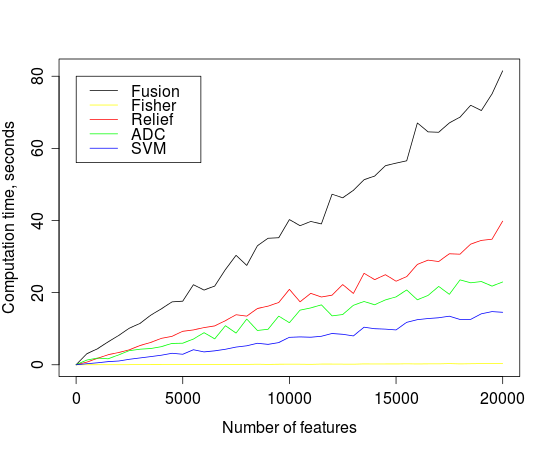
\includegraphics[width=0.7\textwidth]{images/all_performance.png}
 \caption{Pagrindinių dimensijų atrinkimo metodų skaičiavimo laikas.}
 \label{fig:visu_laikas}
\end{figure}
~\ref{fig:cgs_laikas} pavaizduotas konsensuso grupėmis grįsto dimensijų atrinkimo algoritmo skaičiavimo laiko priklausomybė nuo mėginius apibūdinančių dimensijų kiekio. Algoritmo sudėtingumas laiko atžvilgiu yra kvadratinis. Jei lyginsime su dimensijų reitingavimo algoritmais, tai šis algoritmas yra daug kartų lėtesnis.
\begin{figure}
 \centering
 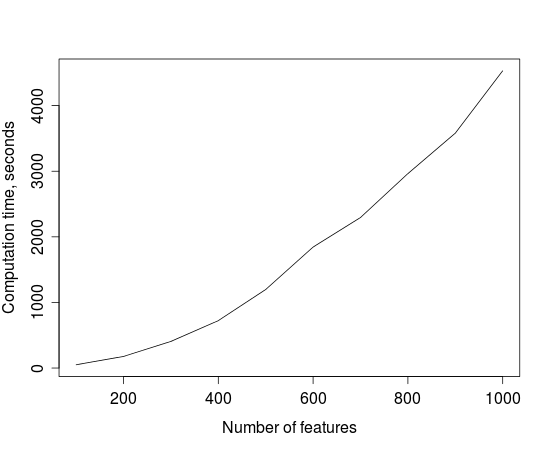
\includegraphics[width=0.7\textwidth]{images/cgs_performance.png}
 \caption{Konsensuso grupėmis grįtas dimensijų atrinkimo metodo skaičiavimo laikas.}
 \label{fig:cgs_laikas}
\end{figure}

Pagal gautus laiko priklausomybės nuo dimensijų kiekio grafikus galime daryti išvadą, kad CGS algoritmas daugiamačių duomenų dimensijų atrinkimui nėra tinkamas, nes darbo laikas yra per didelis.

\subsubsection{Klasifikavimo tikslumas}